% 7
\begin{frame}{Jedna noga jako pierwszy model badawczy}
\begin{columns}[T,onlytextwidth]
\column{0.50\textwidth}
\begin{itemize}
  \item Pełny robot jest trudny: wiele kontaktów, całe ciało, stabilność, opóźnienia.
  \item Jedna noga jest mniejszym, ale nadal wartościowym problemem.
  \item Możemy badać: geometrię, osobliwości, momenty, tarcie i bezpieczne zakresy ruchu.
\end{itemize}
\column{0.46\textwidth}
\begin{center}
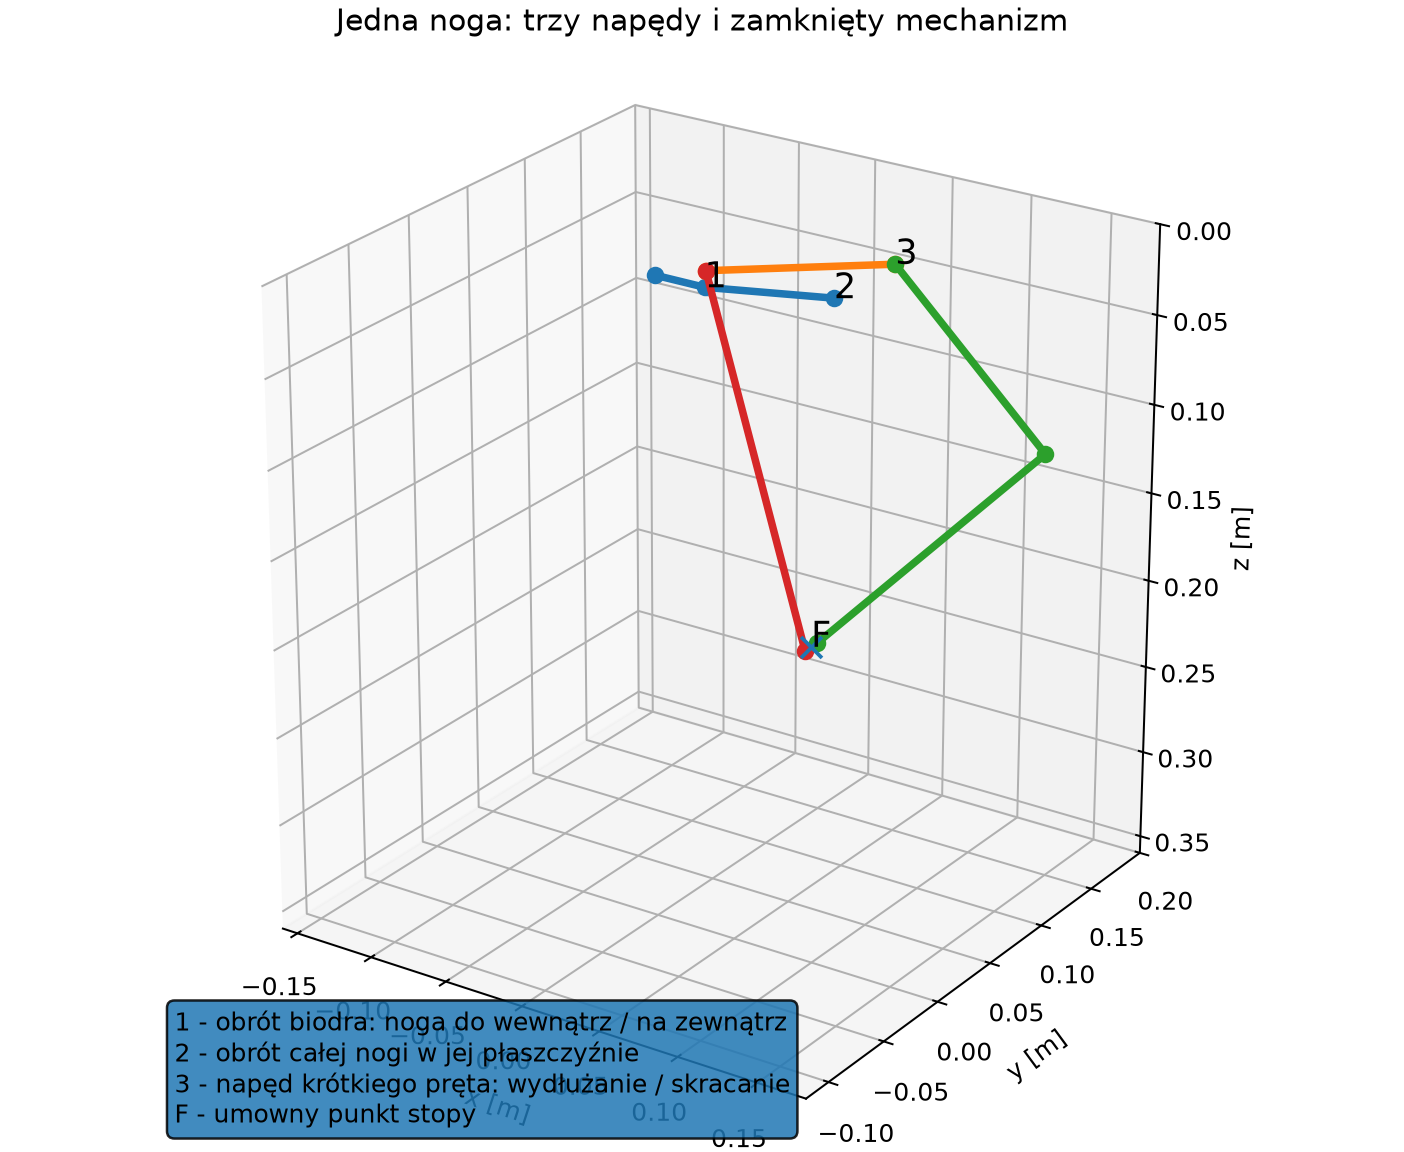
\includegraphics[width=0.9\linewidth,height=0.48\textheight,keepaspectratio]{figures/leg_three_motor_roles_annotated.png}
\end{center}
\end{columns}
\begin{block}{Minimalny cel demonstratora jednej nogi}
Przesunąć stopę do celu, ale nie wejść w konfigurację, z której noga nie może wrócić przy realistycznym tarciu i ograniczonych momentach.
\end{block}
\note{To jest kluczowa zmiana względem wersji z odwróconym wahadłem. Przykład jednej nogi jest bliższy platformie i może być pierwszym niezależnym pakietem badawczym.}
\end{frame}

% 8
\begin{frame}{Trzy napędy jednej nogi: poprawna interpretacja}
\begin{columns}[T,onlytextwidth]
\column{0.56\textwidth}
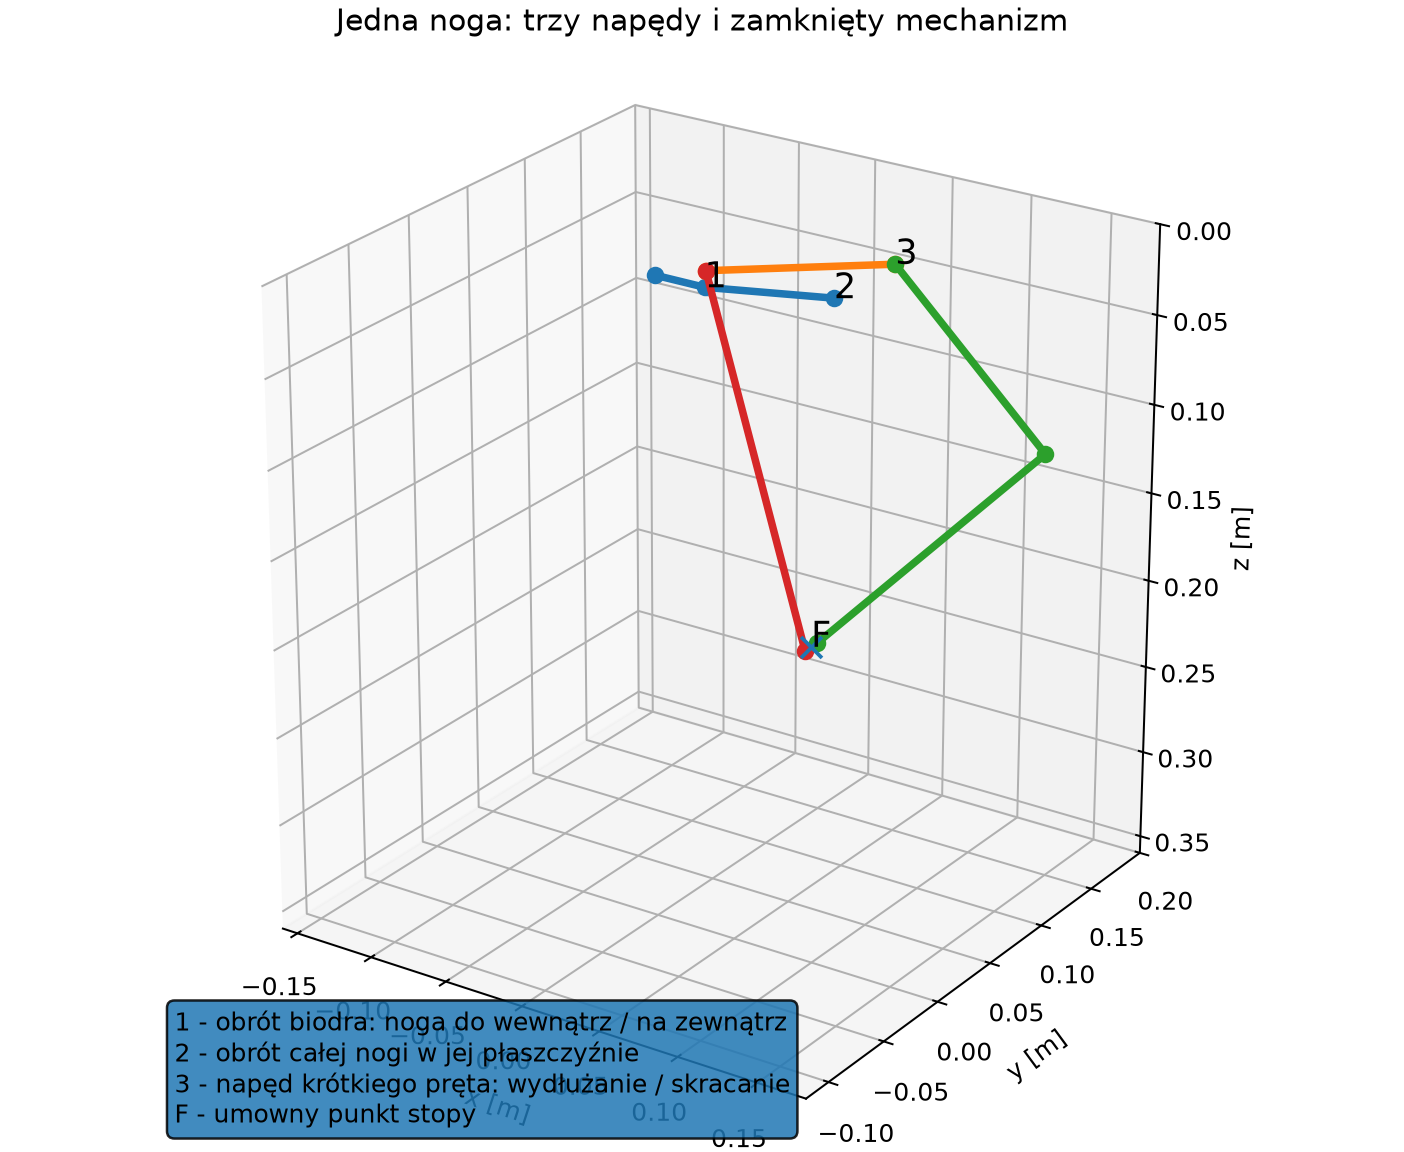
\includegraphics[width=\linewidth,height=0.66\textheight,keepaspectratio]{figures/leg_three_motor_roles_annotated.png}
\column{0.40\textwidth}
\small
\begin{itemize}
  \item $q_{\mathrm{hip}}$: silnik prostopadły do płaszczyzny nogi; ruch biodra do wewnątrz i na zewnątrz od korpusu.
  \item $q_{\mathrm{sweep}}$: obrót całej nogi zgodnie lub przeciwnie do ruchu wskazówek zegara.
  \item $q_{\mathrm{extend}}$: obrót jednego krótkiego pręta czworoboku; zmiana geometrii wydłuża lub skraca nogę.
  \item Dwa pozostałe kąty pętli są bierne i wynikają z jej domknięcia.
\end{itemize}
\end{columns}
\source{Model URDF i kod kinematyki w repozytorium \href{https://github.com/delipl/quadruped_ros2}{delipl/quadruped\_ros2}.}
\note{Poprzedni opis sugerował zbyt ogólnie trzy niezależne przeguby. Tutaj trzeba jasno rozróżnić ruch biodra, obrót całej płaszczyzny nogi oraz napęd krótkiego pręta zamkniętego mechanizmu.}
\end{frame}

% 9
\begin{frame}{Mechanizm czteroprętowy: napęd i kąty bierne}
\begin{columns}[T,onlytextwidth]
\column{0.54\textwidth}
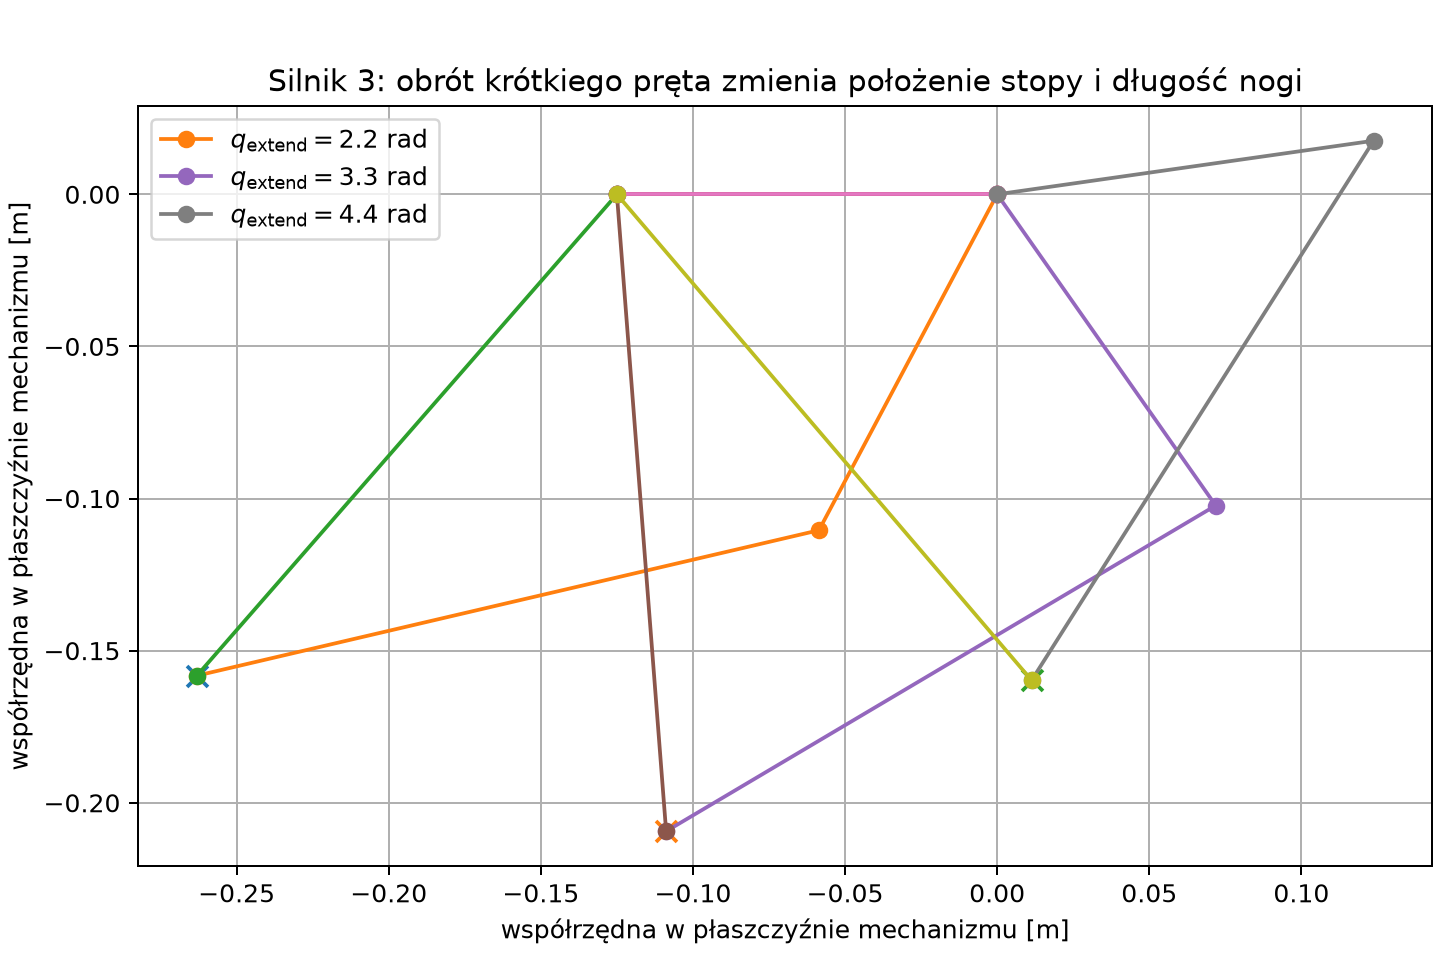
\includegraphics[width=\linewidth,height=0.63\textheight,keepaspectratio]{figures/four_bar_extension_side_view.png}
\column{0.42\textwidth}
\begin{block}{Współrzędne aktywne}
\[
q_a = \begin{bmatrix}
q_{\mathrm{hip}} & q_{\mathrm{sweep}} & q_{\mathrm{extend}}
\end{bmatrix}^{T}
\]
\end{block}
\begin{block}{Domknięcie pętli}
\[
q_p=g(q_{\mathrm{extend}}),
\qquad \Phi(q_a,q_p)=0.
\]
\end{block}
\end{columns}
\note{W kodzie Pythona dwa kąty bierne są rekonstruowane przez bezpośrednią adaptację funkcji update_passive_joints z kontrolera ROS 2.}
\end{frame}

% 10
\begin{frame}{Kinematyka: gdzie jest stopa i jak szybko się porusza?}
\begin{columns}[T,onlytextwidth]
\column{0.50\textwidth}
\begin{block}{Położenie stopy}
\[
p_F = f_{\mathrm{kin}}(q)
\]
\end{block}
\begin{block}{Prędkość stopy}
\[
\dot p_F = J(q)\dot q
\]
\end{block}
\column{0.46\textwidth}
\begin{itemize}
  \item $p_F$ - położenie stopy w układzie robota.
  \item $J(q)$ - macierz Jacobiego: lokalne przełożenie prędkości przegubów na prędkość stopy.
  \item W praktyce $J(q)$ mówi też, czy ruch jest dobrze uwarunkowany.
\end{itemize}
\vspace{0.4em}
\begin{center}
\begin{tikzpicture}[>=Latex,scale=0.95]
  \draw[thick,fill=blue!5] (0,0) circle (0.18);
  \draw[ultra thick] (0,0)--(1.2,-0.8)--(2.1,-1.65);
  \fill[safe] (2.1,-1.65) circle (0.08);
  \draw[->,thick,pwrblue] (2.1,-1.65)--(2.75,-1.25);
  \node[font=\scriptsize] at (2.95,-1.12) {$\dot p_F$};
  \draw[->,thick,warn] (0.25,0.05) arc (10:-50:0.5);
  \node[font=\scriptsize] at (0.8,0.1) {$\dot q$};
\end{tikzpicture}
\end{center}
\end{columns}
\note{To jeden z najważniejszych slajdów edukacyjnych: laik inżynier widzi, że macierz Jacobiego nie jest abstrakcją, tylko lokalnym przełożeniem ruchu napędów na ruch stopy.}
\end{frame}

% 11
\begin{frame}{Osobliwości i utrata „sprawczości” nogi}
\small
\begin{columns}[T,onlytextwidth]
\column{0.52\textwidth}
\begin{itemize}
  \item W dobrej konfiguracji mały ruch napędu daje kontrolowany ruch stopy.
  \item W złej konfiguracji stopa może prawie nie reagować albo wymagać dużego momentu.
  \item W mechanizmach równoległych dochodzą granice geometrii i możliwe złe gałęzie ruchu.
\end{itemize}
\begin{block}{Przykładowy margines}
\vspace{-0.7em}
\[
h_{\mathrm{sing}}(q) = \sigma_{\min}(J(q)) - \varepsilon \ge 0
\]
\vspace{-1.0em}
\end{block}
\column{0.44\textwidth}
\begin{center}
\begin{tikzpicture}[scale=0.82]
  \draw[->] (-0.2,0)--(4.0,0) node[right,font=\scriptsize] {konfiguracja};
  \draw[->] (0,-0.2)--(0,2.1) node[above,font=\scriptsize] {margines};
  \draw[thick,safe] plot[smooth] coordinates {(0.2,1.8)(1.0,1.6)(1.8,1.1)(2.6,0.45)(3.4,0.12)};
  \draw[thick,warn,dashed] (0,0.45)--(3.8,0.45);
  \node[font=\scriptsize,align=center] at (2.5,1.35) {bezpiecznie};
  \node[font=\scriptsize,align=center,warn] at (2.8,0.25) {za blisko\\osobliwości};
\end{tikzpicture}
\end{center}
\begin{itemize}
  \item Dla realnej nogi margines może łączyć geometrię, tarcie i zapas momentu.
\end{itemize}
\end{columns}
\note{Warto powiedzieć, że formuła z minimalną wartością osobliwą Jacobiego jest przykładem. Dla rzeczywistej nogi może być potrzebny lepszy margines: zapas momentu, odległość od limitów, lub miara odzyskiwalności.}
\end{frame}

% 12
\begin{frame}{Dynamika nogi i kontakt z podłożem}
\begin{block}{Ogólny model dynamiki}
\[
M(q)\ddot q + C(q,\dot q)\dot q + g(q) = B\tau + J_c(q)^T f_c
\]
\end{block}
\begin{columns}[T,onlytextwidth]
\column{0.48\textwidth}
\begin{itemize}
  \item $M(q)$ - bezwładność.
  \item $C(q,\dot q)\dot q$ - efekty zależne od prędkości.
  \item $g(q)$ - grawitacja.
\end{itemize}
\column{0.48\textwidth}
\begin{itemize}
  \item $\tau$ - momenty napędów.
  \item $f_c$ - siły kontaktu stopy z podłożem.
  \item $J_c(q)^T f_c$ - przełożenie sił kontaktu na przeguby.
\end{itemize}
\end{columns}
\begin{block}{Poziom dokładności}
Dokładny model jest potrzebny do walidacji; model sterowania czasu rzeczywistego może być uproszczony, ale musi zachować kluczowe ograniczenia.
\end{block}
\note{To nie ma być wykład z mechaniki analitycznej. Slajd ma pokazać, które zjawiska trzeba uwzględnić, kiedy z pozycji stopy przechodzimy do momentów silników i realnego kontaktu.}
\end{frame}
